\section{Method} \label{sec:method}
%Method
%Prerequisites (things used by all networks)
%Data set (fruit), (landscape)
%Input size (128X128)
%
%Color spaces + which one to use :
%RGB (luminosity not separated from color)
%HSV (circular domain)
%YCbCr (OK)
%CIELab (OK)
%first layer as input, second and third layer as output
%
%Architecture (not what it is but why WE use it)
%General discription (how to colorize an image with an NN)
%Features used by all networks
%ReLu, weight initialization, padding, kernel size
%Feature extraction
%Reconstruct
%Concatenate
%Dilated convolution
%Color generation
%Two feature maps
%blur
%Classification
%k-means
%annealed mean
%gaussian blur
%
%Loss function
%Squared error
%Class rebalancing (histogram dataset)
%Cross entropy
%Class rebalancing
%Architectures used:
%Dahl, Compact, Dahl_classifier, Dahl_zhang, Zhang
%
%Training method
%nesterov momentum
%adadelta

This section covers the different methods used to get an answer to the question of which CNN setup is best in colorization of images. Firstly, the chosen dataset will be explained. In addition the input size and the different colorspaces used will be explained. Next the different architectures used will be explained. Features extraction, training parameters, loss functions, and general architectures of the chosen networks will be evaluated. Finally the test setup will be explained.

\subsection{Dataset and Input}

Large training and validation datasets are required for training and validation of the CNNs.
Some restrictions on the datasets had to be made due to limitations in computational power, resulting in a selection of images based on a certain category; fruit and landscape images.

The landscape dataset is used as a low-level test case, images of landscapes offer less distinct features coupled to a mapping of the colors, e.g. most landscapes are green at the bottom and blue at the top. The high-level test case consists of the fruit dataset.
Fruit is a category which has distinct colors corresponding to distinct features. Therefore, in order to color fruit correctly, the network has to learn to link colors to distinct features in the input, straining the networks requirements. Also many fruit classes are linked to ambiguous colors, i.e. green or red apple. Taking fruit as the dataset is therefore an excellent method to check whether the network is able to counter the 'averaging' problem also mentioned before.

The datasets are generated using the popular image website Flickr\footnote{\url{https://www.flickr.com/}}.
Using their freely available API, a program was made that retrieved images in the required resolution and kept track of images retrieved, to avoid duplicates. The datasets retrieved had to be checked on incorrect images. To solve this problem a web application was made that enabled us to check images on defects. The checked datasets are collected in batches and stored in Python Numpy arrays as input for the network.
This resulted in 2 datasets, which are summarized in table \ref{tab:dataset}.

\begin{table}[h!]
	\centering
	\caption{Datasets used for training and validation of the various networks}
	\label{tab:dataset}
	\begin{tabular}{|l|l|l|}
		\hline
		\textbf{Dataset}   & \textbf{\# Training Images} & \textbf{\# Validation images} \\ \hline \hline
		Fruit\footnote     & 12000            & 2000              \\ \hline
		Landscape & 34000           & 5000              \\ \hline
	\end{tabular}
\end{table}

\footnotetext[2]{The dataset contains  out of 7000 original images, it is doubled in size by mirroring the images around the y axis.}

The images in the fruit dataset are mirrored to increase the dataset. The network input are 128x128 pixel grayscale images, which are propagated through the network in batches. Using batches reduces computation time since better use is made of the parallelization of modern computer architectures. Most importantly the gradients calculated using batches are a better estimate of the gradient for the entire training set, thus leading to a more stable gradient descent \cite{ioffe2015batch}. Making the batch size too large makes the search to the global minimum less stochastic, thus making it converge to a local optimum more quickly, and in general converging less quickly. \\

\subsubsection{Colorspace}
Different colorspaces can be used for training of the CNNs, the options available are described below.\\


%The network is trained to be able to colorize an image, but the way it outputs the colorized image is dependent on the color space used during training. There are several options available:\\

\textbf{RGB} This widely used color space specifies an intensity for the channels red, blue and green. The biggest drawback of using RGB is that the color is not separated from the luminosity. In this way, the network needs not only to output a hue and saturation of a color, but also the luminosity itself. This makes it a much tougher challenge to output an image that resembles a colorized version of the grayscale image. A visualization of the RGB space is given in figure \ref{fig:RGB}.

\textbf{HSV} Specifying the hue, saturation and value, uncouples the luminosity (value) from the color (hue and saturation). Furthermore decoupling the saturation could allow specifically tackling the sepia and saturation problem as described in section \ref{sec:intro}. However, the color space is periodic in the hue axis. From the numerical perspective, this leads to an ambiguous error specification, since for one difference between target and network output color, two directions of improvement are equally valid, thus a very complicated loss function is required, where the network needs to learn this circular property of the hue axis. This colorspace is used for training on the compact network architecture, however the network did not perform as good as when it was trained on either YCbCr or CIELab. Therefore the HSV colorspace was omitted.

\textbf{YCbCr} The Y channel contains the luminosity of the image, while Cb and Cr layers are the chroma blue and chroma red layers respectively. While providing a separate luminosity channel, it was found that for different Y values, a given Cb and Cr combination does not specify the same color. This makes the error in the color specification dependent on the luminosity of the image. A visualization of the color space can be found in \ref{fig:YCbCr}.

\textbf{CIELab} Similarly to the YCbCr color space, the L channel specifies the luminosity, the a and b layers the color. In contrast with the YCbCr space, a given a and b value specify a color, while the luminosity only determines how light the color is. However, for a single L layer not all a and b value translate to colors that can be represented in the RGB color space (as displayed by computer monitors). The CIELab color space is visualized in figure \ref{fig:CIELab}.\\

To summarize, the HSV, YCbCr and CIELab color spaces all have the possibility of using one channel as input to the neural network, while requiring only two outputs of the network that instead of three with the RGB color space. Combined with the input, these two outputs allow reconstructing a color image. According to Iizuka, the CIELab color space has been found to give the most correct results for a colorization network\cite{IizukaSIGGRAPH2016}. Considering the disadvantages of the HSV color space, the YCbCr and CIELab color spaces are compared during the present research.

\begin{figure}
	\centering
	\begin{subfigure}[b]{0.32\textwidth}
		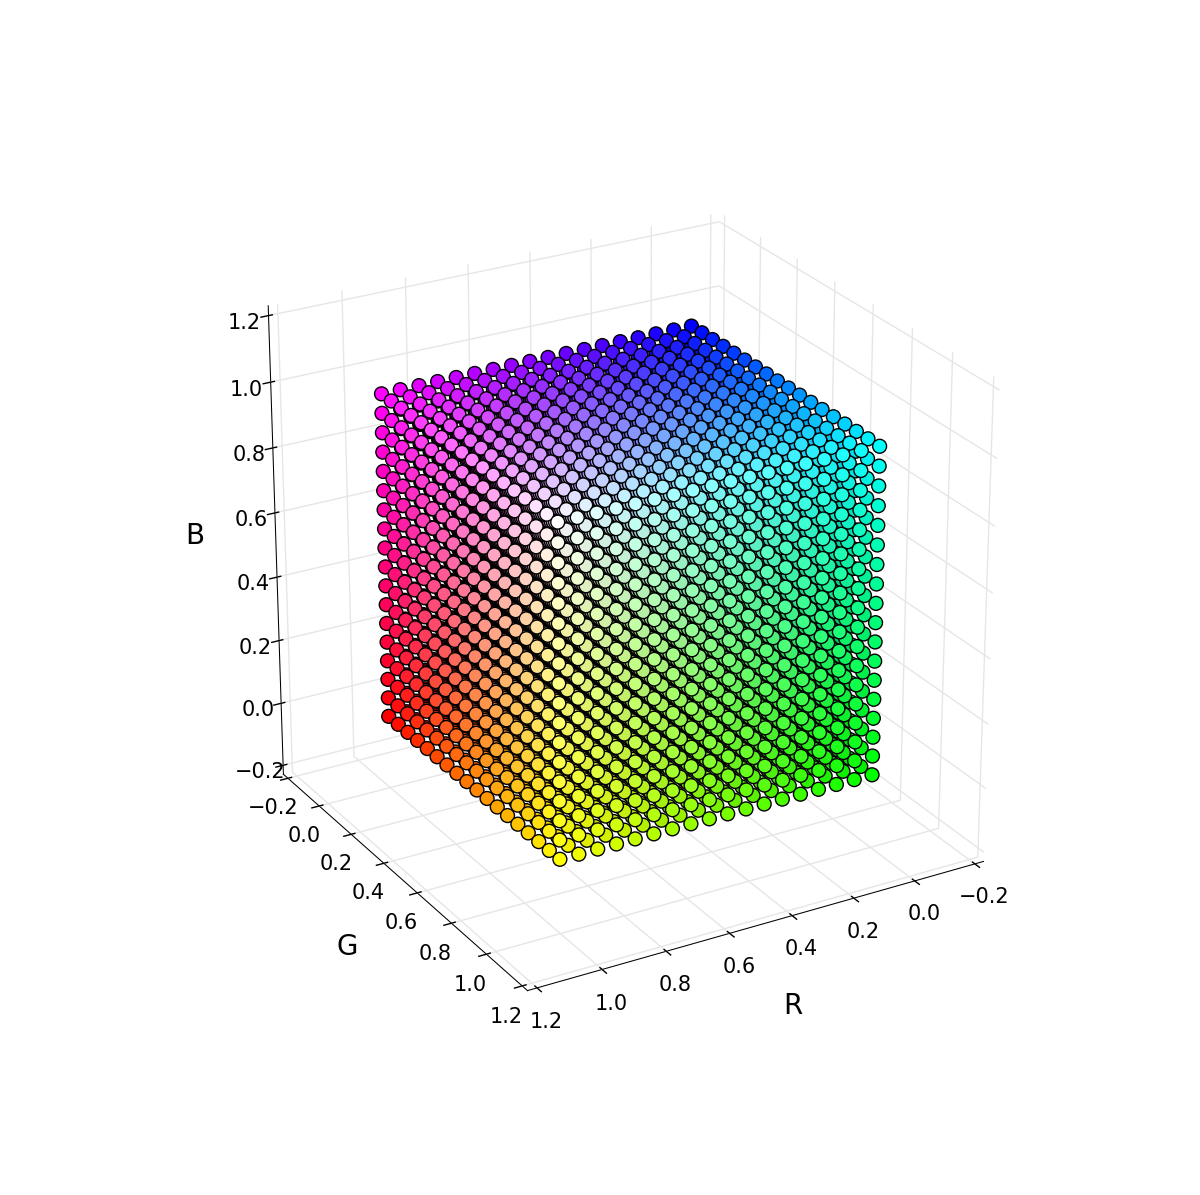
\includegraphics[width=\textwidth,trim={125px 75px 125px 75px},clip]{RGB}
		\caption{The RGB colorspace}
		\label{fig:RGB}
	\end{subfigure}
	~ %add desired spacing between images, e. g. ~, \quad, \qquad, \hfill etc. 
	%(or a blank line to force the subfigure onto a new line)
	\begin{subfigure}[b]{0.32\textwidth}
		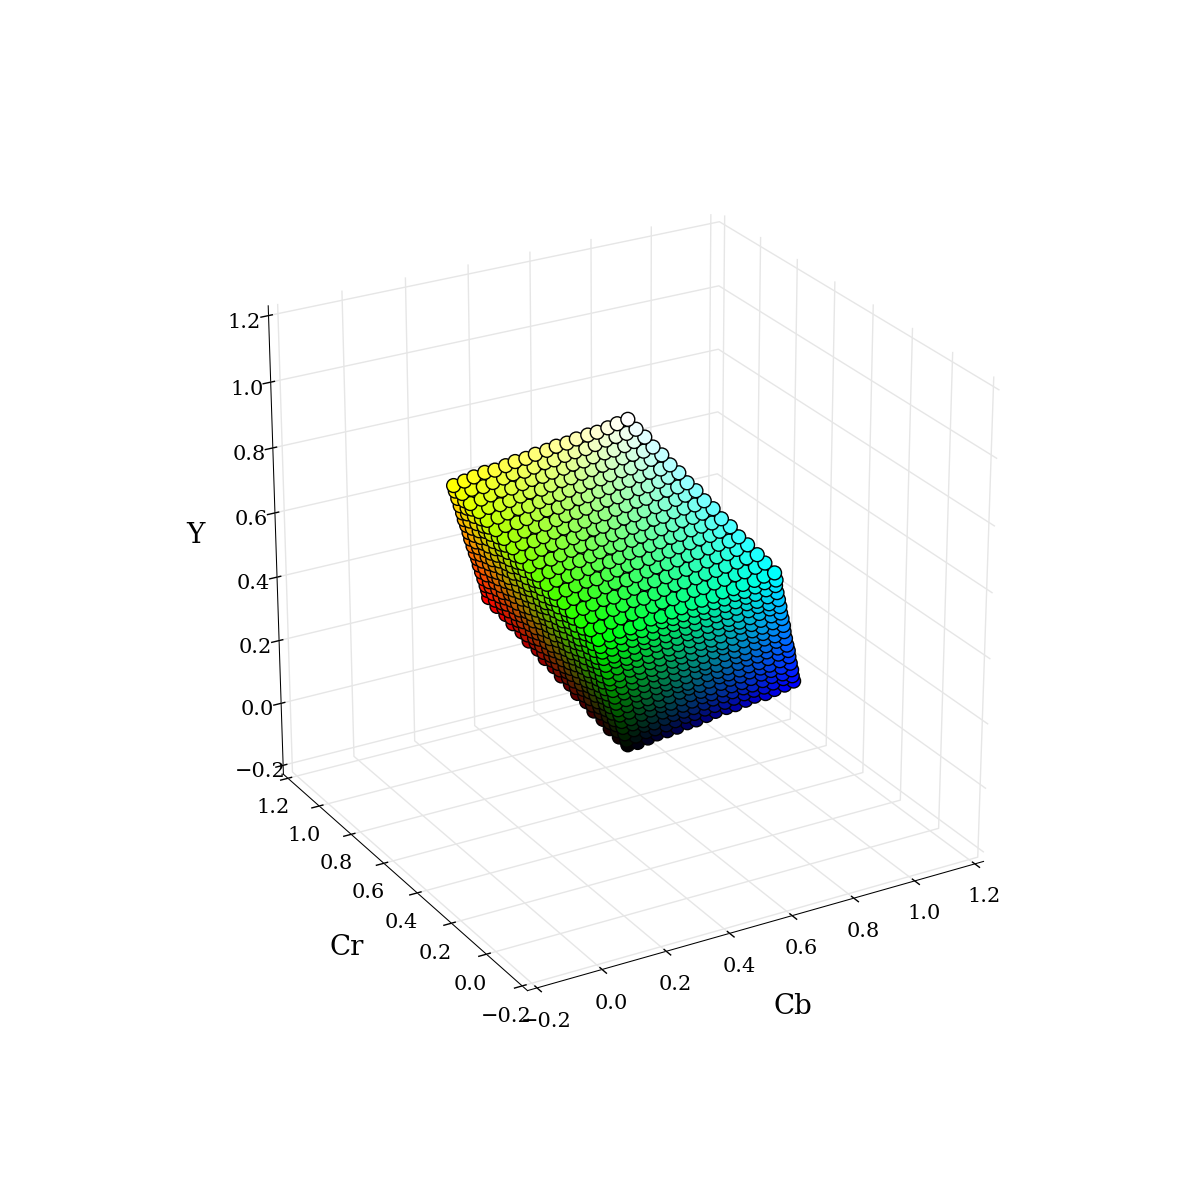
\includegraphics[width=\textwidth,trim={125px 75px 125px 75px},clip]{YCbCr}
		\caption{The RGB colorspace represented in the YCbCr colorspace}
		\label{fig:YCbCr}
	\end{subfigure}
	~ %add desired spacing between images, e. g. ~, \quad, \qquad, \hfill etc. 
	%(or a blank line to force the subfigure onto a new line)
	\begin{subfigure}[b]{0.32\textwidth}
		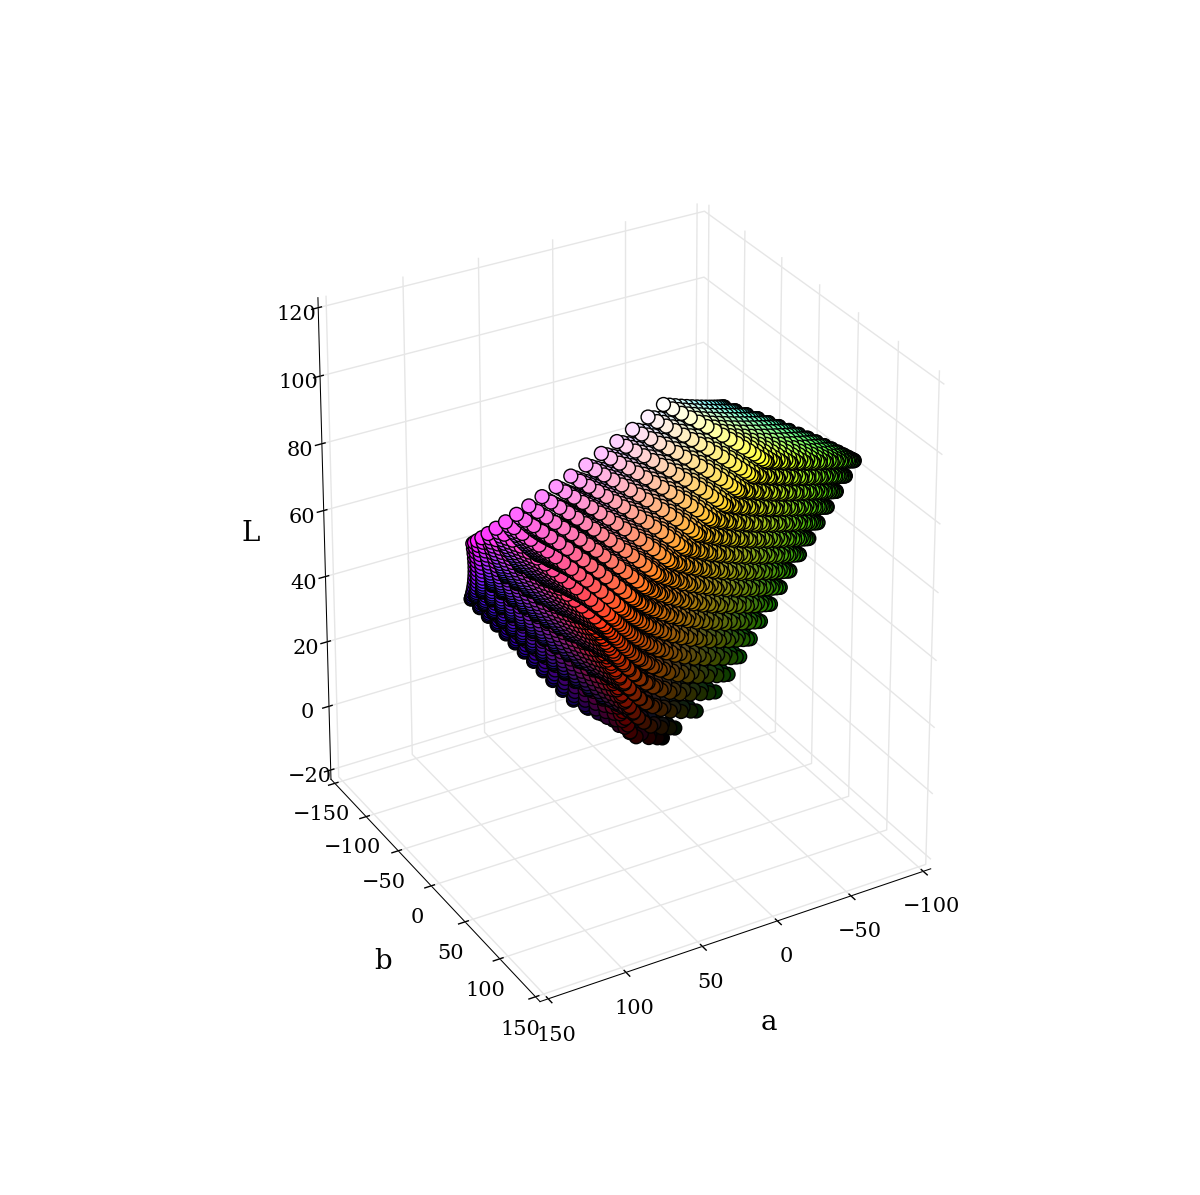
\includegraphics[width=\textwidth,trim={175px 75px 150px 75px},clip]{CIELab}
		\caption{The RGB colorspace represented in the CIELab colorspace}
		\label{fig:CIELab}
	\end{subfigure}
	\caption{The different colorspaces used in the different networks}\label{fig:animals}
\end{figure}

\subsection{Convolutional neural network properties}
\label{sec:nnproperties}

Convolutional neural networks contain a vast amount of properties that determine the behaviour of the network. Structure of the loss function and the model architecture being the most important properties. To compare different architectures, it is important to keep the hyperparameters the same as much as possible, resulting in a fair comparison between CNNs. The choices made in the experiment setup which are affiliated with the CNN properties will be explained here.

A few parameters are held constant over all the test cases. The parts of the network (or the complete network) that are initialized without pre-trained weights are randomly initialized. This is done using a Glorot Uniform distribution \cite{Glorot}. This weight initialization method samples from a uniform distribution with its variance scaled depending on the ingoing and outgoing data. 

The intermediate layers of all the network consist of convolutional layers. All convolutional layers use ReLu non-linearities \cite{nair2010rectified}, except for the final output layers, they are different per architecture. 
Kernel sizes in the convolutional layers of the network are of size 3x3. This kernel size is based upon VGG16's \cite{Simonyan} kernel size, as is used in the other reference networks \cite{Dahl}\cite{Zhang} \cite{ioffe2015batch}.
Stride in the convolutional layers is 1x1 by default. However, in the CNNs using dilation in the output pipeline, stride is used as a way to downsample the resolution of the image, comparable to the function of max pooling, but retaining more spatial properties of the input image \cite{yu2015multi}. Padding is required when using convolutional layers due to the fact that border information of the image is lost when convolving. This property is set to keep the output resolution the same as the input resolution. Zero valued padding is used when conventional convolutions operations are performed. Symmetric valued padding is used when dilated convolutions are used, again the amount of padding is chosen to keep the output dimensions the same.\\


\subsubsection{Feature Extraction}
To recognize certain objects in grayscale images, object dependent features are extracted. This is done in the first part of the convolutional neural network, also known as the input pipeline. To extract features convolutional layers are used. Each convolutional layer convolves the input of the layer with a kernel to a set of feature maps. Max-pooling is often used to make feature extraction spatially invariant to input transformations \cite{Simonyan}. The kernels in the incoming pipeline of the CNN can be chosen to be initialed from scratch, or to be initialed with pre-trained weights. For example VGG16 \cite{Simonyan} has shown excellent results in image classification, and therefore already has a large amount of feature extraction available. In this paper a comparison is made between using architectures which are completely trained from scratch, and architectures which use the input pipeline of the VGG16 network to initialize the convolutional kernels.\\

\subsubsection{reconstruction}
In the input pipeline of the network, the image is reduced to a set of features, containing decreased amounts of spatial information. To be able to colorize the image, localization of these features is required. The feature maps can be upscaled using linear upscaling. There are multiple ways of retrieving the spatial information of the image \cite{Charpiat} \cite{Zhang}. The methods tested in these paper consist of residual auto-encoders and dilated convolutions \cite{yu2015multi}.

The use of a residual auto-encoder has been demonstrated by \cite{Dahl}. After the bottleneck of the CNN each layer is upscaled and concatenated with the parallel layer in the input pipeline of the network. This way global features are merged with the localization of those features. This process is repeated after each upscale layer until the output of the network is reached, as can be seen in figure \ref{fig:dahlnetwork}.

%This is done by concatenating the layers of the same resolution before the bottleneck with the upscaled features after the bottleneck. Then an convolutional layer is used to merge these features in feature maps of the upscaled resolution. This process is repeated until the original image resolution is retrieved.
%
Another technique used is the use of dilated convolutions \cite{yu2015multi}. Zhang et al. use strides for downsampling in the incoming pipeline of the CNN, which causes less loss of spatial information. The bottleneck of the network consists of 28x28 feature maps. The output pipeline of the network is initialized by two layers of dilated convolutions, where each layer consists of 3 consecutive dilated convolutions. Using dilated convolutions has the effect that the input pipeline can compress the image to a larger size leaving more spatial information in the bottleneck of the image. The receptive field of dilated convolutions grows exponentionally with an increase in layers, as opposed to linearly with conventional convolutions. Less consecutive convolutions are therefore required when dilated convolutions are used in comparison with conventional convolutions.\\


\subsubsection{Color Generation}
In the final layers of the network, the original image color layers have to be reconstructed. Two different methods are used throughout the paper: construction using two feature maps and classification.

Construction using two feature maps is a direct result of retrieving the original image resolution through the reconstruction of the image. As a final layer, a convolutional layer is used that maps to two feature maps, which represent the two color layers that are finally used to create a colorized image.

\begin{wrapfigure}{R}{0.5\textwidth}
	\vspace{-20pt}
	\begin{center}
		\includegraphics[width=0.40\textwidth,trim={75px 0px 75px 0px},clip]{K_nearest}
	\end{center}
	\caption{An illustration of the K-nearest neighbour algorithm. The red dots represent the centers of the colorbins in the discretized colorspace. The blue dot represents the ground truth ab value of the target pixel. The yellow dots correspond the the K-nearest neighbour colorbins. The class probabilities of the targetvector are generated by applying a gaussian blur on the distances to the K-nearest neigbour colorbins.}
	\vspace{0pt}
	\label{fig:k_nearest}
\end{wrapfigure}

As an aid to the colorization process, a Gaussian Blur is used on the color layers of the original image. Colorization does not require precise pixel by pixel colorization, because colors in images mostly appear in sets of pixels. When blurring, this enables the network to more easily converge towards a solution by reducing the noise in the color of the pixel set, i.e. a mapping between a texture and a color is created in the network, without too much regard for the texture in the color layers. Note that blurring the color layers does not reduce the image fidelity. This is due to the fact that the luminosity layer contains the details and contrast of the image, which is subsequently merged with the output color layers of the network. To the human eye, a blurred a and b layer with an unblurred L layer makes for an image that is almost indistinguishable from the original image. A comparison between different grades of blurring is made and shown in the section \ref{sec:results}. Mapping an L layer directly to an a and b layer makes the colorization problem into a regression problem, where a continuous function is sought which maps a grayscale input to the two values that determine color in the output.

The other method used is a classification approach to colorization: for a given input image, every pixel in the output image falls within one of a few predefined color classes. For the classification networks, the colorspace CIElab is used. The ab colorspace is discretized into $n$ classes, each corresponding to a discretized bin in the original ab colorspace. Classification applies a loss function per pixel in the image, so each pixel has a corresponding target vector. Instead of generating one-hot vectors per pixel, probability distributions are generated, assigning probabilities to multiple colorbins. This way the network can make use of the similarity of different colors in the ab colorspace. Using a target vector which has a distribution over the classes instead of a one-hot vector, helps to steer the network to the correct colors. In addition the use of a color distribution more closely resembles the nature of the colorization problem, since not every object is linked to a single color, but rather a distribution of possible colors. 
Each target vector is generated by applying a gaussian blur over the k-nearest neighbour colorbins of the exact ab value, as can be seen in \ref{fig:k_nearest}. The result of these operations over one image is a set of $128*128=16384$ target vectors, each consisting of a probability distribution over the $n$ colorbins. 

\begin{figure}[h]
	\centering
	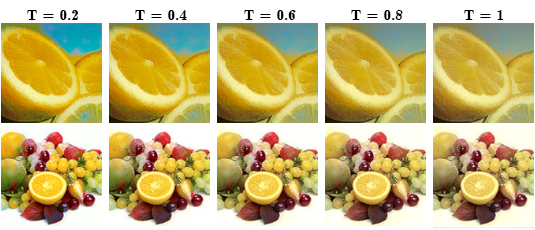
\includegraphics[width=0.59\textwidth]{AnnealedMean.jpg}
	\centering
	\caption{Effect of applying the annealed mean operation on the  color output probabilities of the network. Lowering the T brings out more vibrant colors in the image. A higher T will results in more dull colors.}
	\label{fig:anmean}
\end{figure}

The final colorized version of the image is created by processing the probability distribution per pixel. Implementing an annealed mean to pick the best color from the probability distribution allows setting the degree with which to pick either the mode or the mean of the distribution \cite{Zhang}. The annealed mean operation can be seen in table \ref{eq:anmean}, where \textbf{z} is the output probability vector of one pixel, T is the annealed mean temperature, and q is the total number of colorbins. Both the two feature maps and classification approach are tried during the present research.\\




\subsubsection{Loss Function}
During the present research, several loss functions were used, depending on the color generation method used.
The two feature maps represent the color space layers of the to be reconstructed image, depending on the selected colorspace. The loss function is then defined as the sum of the squared distances between the output of the network and the original image color layers. This can be seen in equation \ref{eq:squaredsum}, where $p$ is the prediction of the network, $t$ is the target, $H$ and $W$ denote the pixel index, and $W$ denotes the channel. The distances are calculated per pixel and per color channel.

\begin{equation}
\label{eq:squaredsum}
L = \sum_{H}\sum_{W} \sum_{C}(p - t)^2
\end{equation}

To enable the network to use more saturated colors, color rebalancing may be applied to the loss function. This color rebalancing penalizes the the network for selecting desaturated colors, by exponentially increasing the loss function when converging towards desaturated solutions. However, it was found that this does not produce desired results, probably due to the fact that it makes no use of the actual probability of the colors, thus leading to a crude approximation of the histogram. For the two feature maps output, the standard sum squared error as in equation \ref{eq:squaredsum} is used.

\begin{equation}
f_{T}(\textbf{z})=\frac{exp(\textbf{z}/T)}{\sum_q^{}exp(\textbf{z}_{q}/T)}
\label{eq:anmean}
\end{equation}\begin{wrapfigure}{R}{0.5\textwidth}
	\vspace{-20pt}
	\begin{center}
		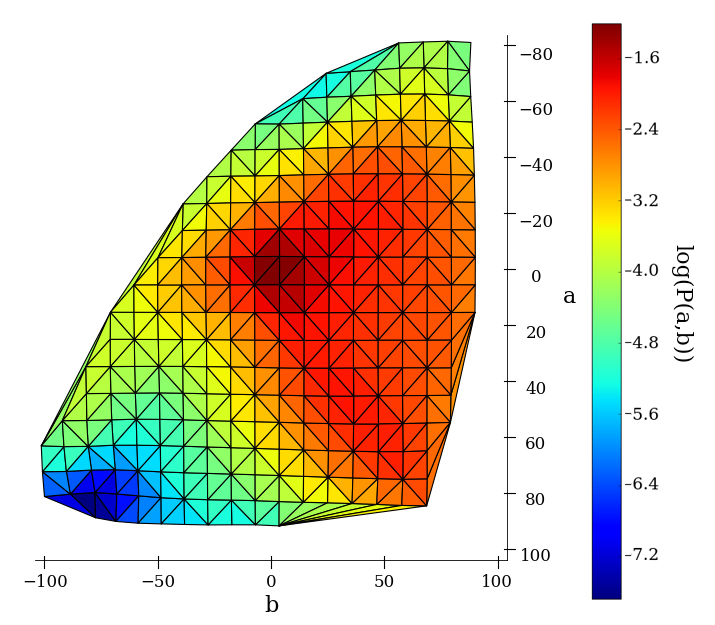
\includegraphics[width=0.48\textwidth]{hist}
	\end{center}
	\caption{Histogram of the total fruit dataset. It can be seen that the colors are heavily biased towards positive $b$ values. Also two ridges can be identified corresponding to more green and red colors. This comes from the large amounts of strawberries and leaves in the dataset.}
	\label{fig:histogram}
	\vspace{20pt}
\end{wrapfigure}

For classification, categorical cross-entropy is used. This is done between the predicted color classification of the network per pixel and the target classification per pixel of color layers of the image. The categorical cross-entropy function is defined in equation \ref{eq:crossentropy}, where $t_{i,j}$ is the target classification, where $i$ specifies the pixel, and $j$ its respective probability distribution of the classified color. 
$p_{i,j}$ is the predicted classification, where $i$ depicts the predicted pixel. $j$ its estimated probability distribution of the classified color, by the network.

\begin{equation}
\label{eq:crossentropy}
L_{i} = -\sum t_{i,j}\log(p_{i,j})
\end{equation}

Due to the fact that in the training set the lower a and b values are highly represented, after training a bias will result towards picking lower a and b values during colorization, thus leading to under saturated results. 
Class rebalancing is added to assist the network in coping with this existing skewness of the training data set. This is done by generating a histogram of the discrete colors in the dataset. The histogram is used to balance the loss function with respect to probability of each color. The histogram of the dataset can be found in figure \ref{fig:histogram}. The  histogram is mixed with a uniform distribution with uniform factor $\lambda$. A $\lambda$ value of 1 means no class rebalancing, a $\lambda$ value of 0 means full class rebalancing. The final value function is normalised to be one on expectation. The class rebalancing factor is given by equation \ref{eq:classrebalance}, where $H$ is the histogram of the dataset, $\lambda$ is the uniform mixing factor and $q$ is the target vector containing the color probabilities. The complete loss function of the cross-entropy is given by equation \ref{eq:lossZhang}.

\begin{equation}\label{eq:classrebalance}
v(q) = ((1 - \lambda)\cdot H + \lambda)^{-1} \cdot q
\end{equation}
 
\subsection{Training method}
For convolutional neural networks training, stochastic gradient decent (SGD), sometimes together with momentum, is commonly used for updating the weights and biases \cite{IizukaSIGGRAPH2016}\cite{Simonyan}. The used hyper-parameters, especially the learning rate, requires careful tuning when using SGD. Often a scheduled learning rate, that is monotonically decreasing depending on the epoch, results in the best results. Since the focus of the present research lies not on what training method parameters are required, ADADELTA was used to automatically set the learning rate for every parameter\cite{zeiler2012adadelta}. Furthermore, Nesterov momentum was applied to lower the probability of getting stuck in a local minimum\cite{sutskever2013importance}.

\subsection{Final choice of model architectures}
In order to test the different architecture features as described above, five different neural network model architectures were designed. These architectures are implemented and tested for their performance. A summary of the architectures hyperparameters and properties used in the experiments can be found in table \ref{tab:architectures} in appendix \ref{ap:NNset}. All of the network architectures are described how and why they differ from the other architectures. The networks are also illustrated in different figures, for which the legend, in which the different layer are explained, is found in figure \ref{fig:Legend}.
The different options for the networks are all described in the rest of the method section, but a short summary is given here:\\

\begin{itemize}
	\item Feature extraction: use a non-pretrained net or the input pipeline of VGG16.
	\item Color generation: use a two feature map output as used by Dahl \cite{Dahl} and Iizuka et al. \cite{IizukaSIGGRAPH2016} or a classification approach as done by Zhang \cite{Zhang}.
	\item Feature extraction downscaling: Use max-pooling as used by Dahl \cite{Dahl} or a stride in the convolutional filter as used by Zhang and Iizuka \cite{Zhang}\cite{IizukaSIGGRAPH2016}.
	\item Reconstruction of local features: use concatenation and upscaling, leading to a form of hypercolumns as explained by Dahl \cite{Dahl} or dilation as used by Zhang \cite{Zhang}.
\end{itemize}

\begin{figure}[h!]
	\centering
	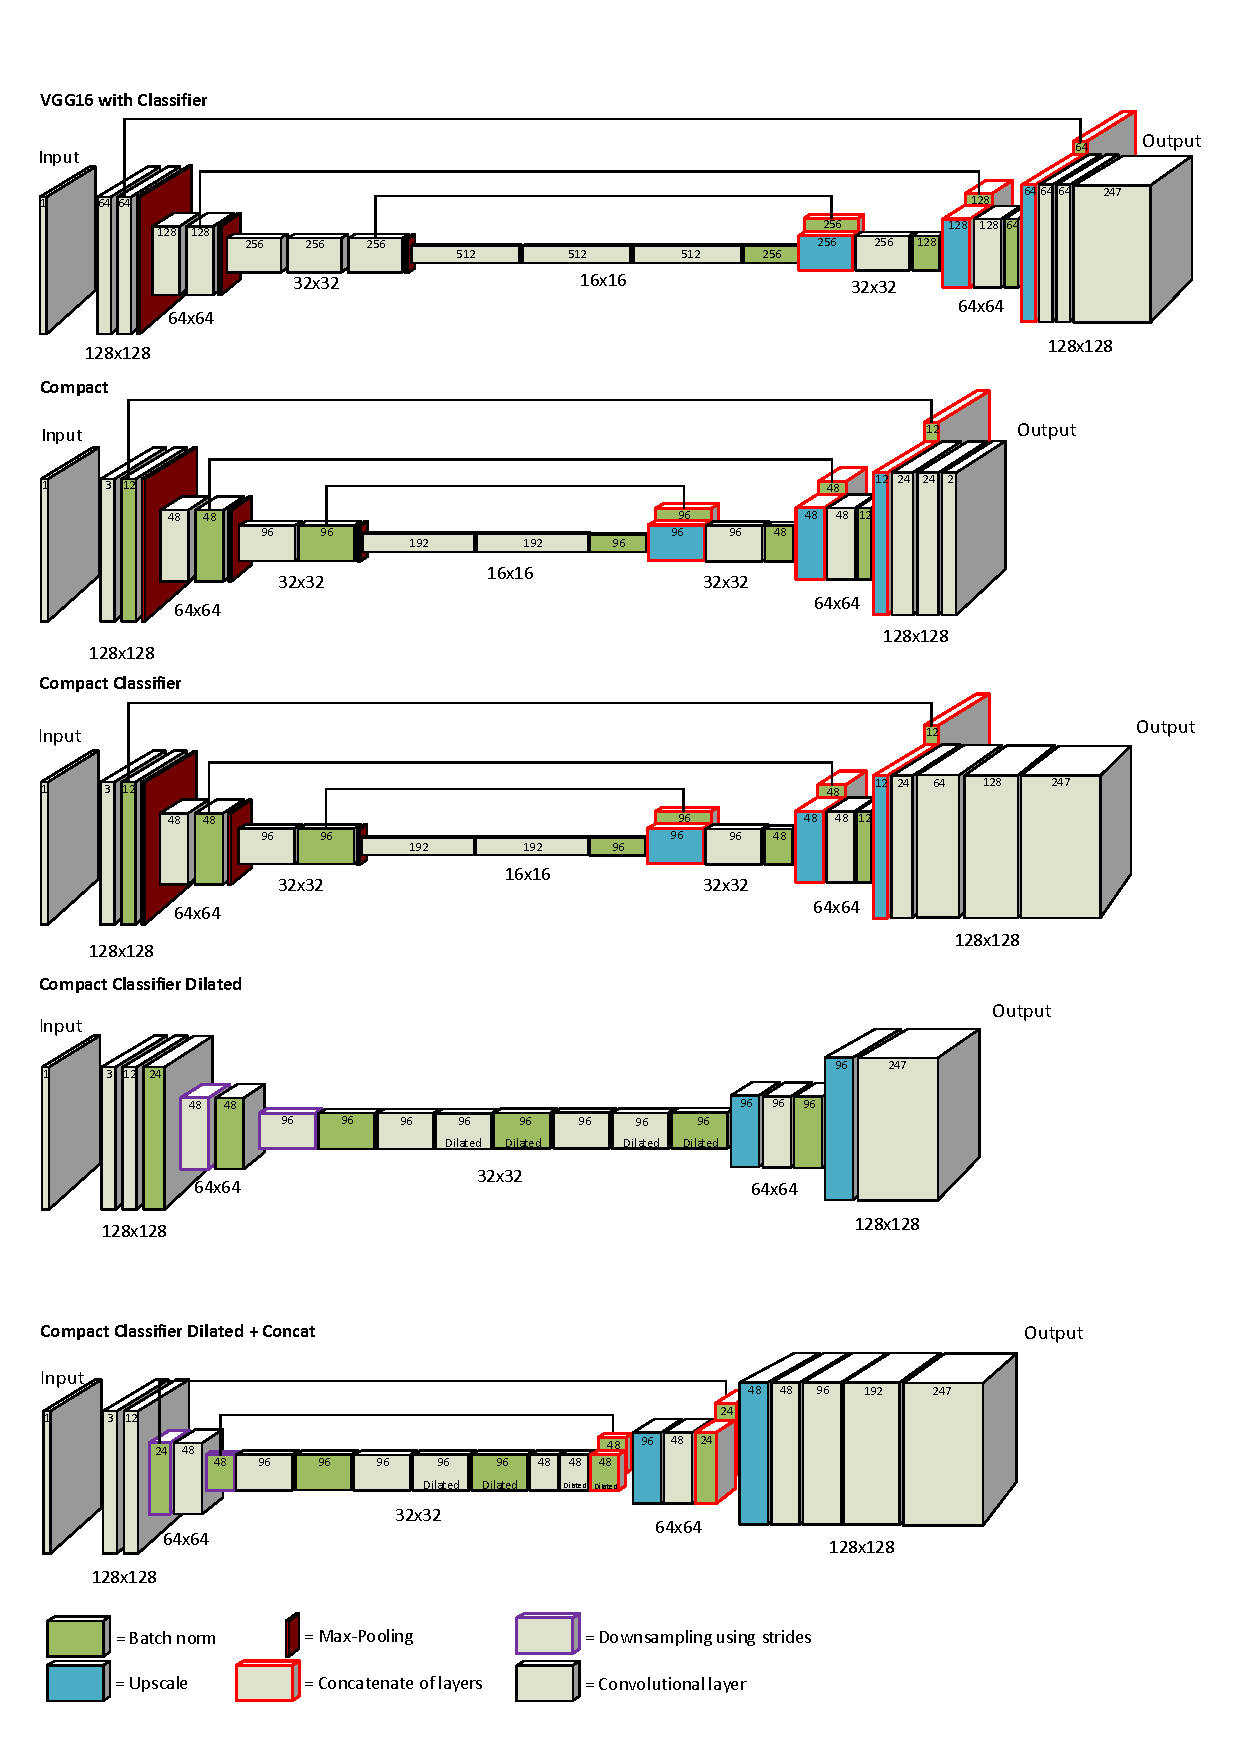
\includegraphics[width=0.9\textwidth,trim={0cm 0.5cm 7cm 26.9cm},clip]{final_architecture.pdf}
	\caption{The legend specifying all the different layers used in the architectures. The batch normalization layer is a convolutional block with batch normalization done before applying the non-linearity. Max pooling is a non-trainable layer that reduces the image size inside the network. Downsampling using strides, is a convolutional layer block with strides applied to reduce the image size. Upscale layer, is upscaling applied after which a convolutional block follows. The concatenate block, can consist out of different other layers, the possible batch norm or upscale operations are applied from each block before they are concatenated, after which a (dilated) convolution layer follows.}
	\label{fig:Legend}
\end{figure}

\subsubsection{Compact}
The compact network is the only network that does not use classification as the color generation part of the network, but rather the two feature map output. Max-pooling is used for downscaling and concatenation as its way of retrieving the spatially local information. Furthermore it is trained with randomly initialized weights. The network architecture is illustrated in figure \ref{fig:compact}. One thing to note is that in the last layer in the bottleneck a 1x1 kernel is used in the convolution. This to reduce the number of feature maps such that there is an equal amount of features concatenated between the more local and the global features.
\begin{figure}[H]
	\centering
	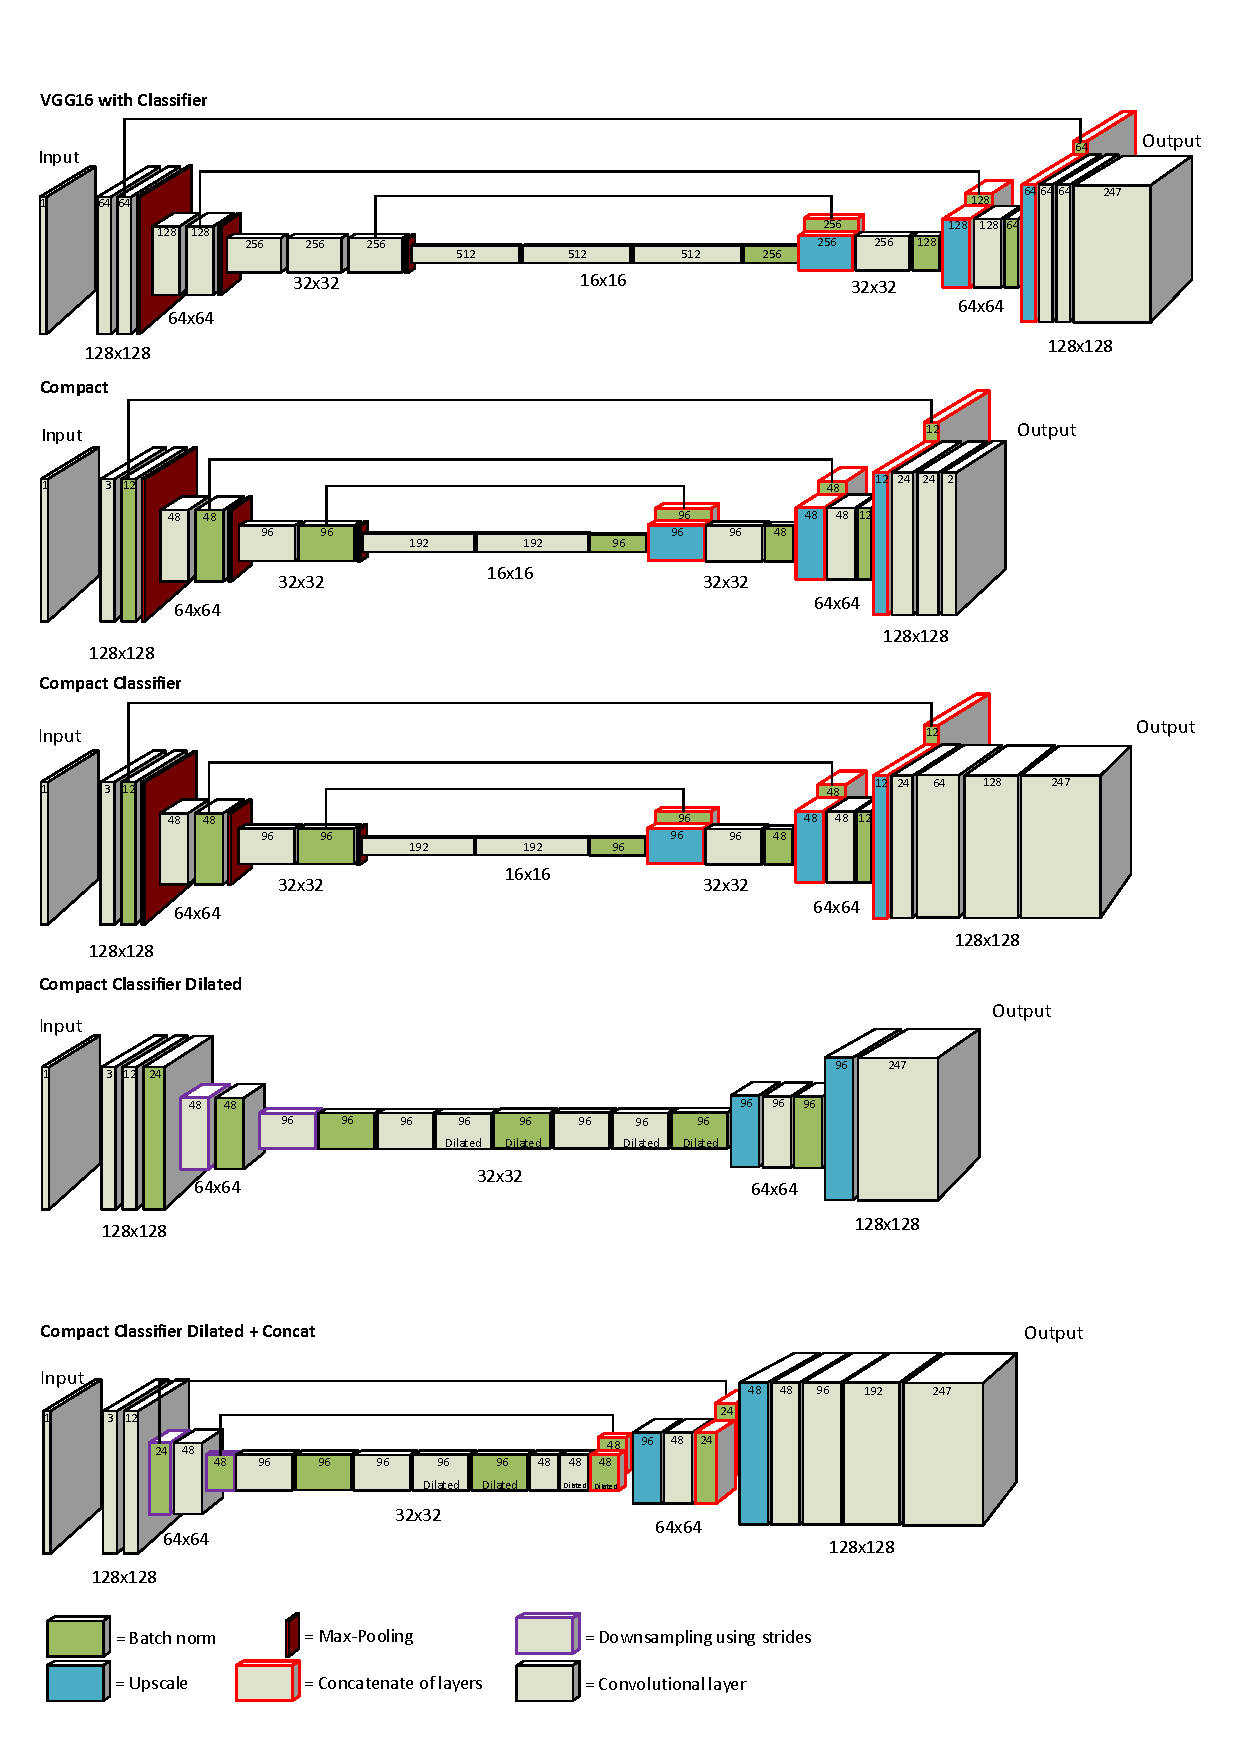
\includegraphics[width=0.88\textwidth,trim={0cm 17.97cm 2.5cm 6.3cm},clip]{final_architecture.pdf}
	\caption{The compact network architecture. The black lines illustrate which layer is concatenated with which layer in the reconstruction part, and are visually stacked on top of the more local feature maps. The definition of each different layer can be found in figure \ref{fig:Legend}.}
	\label{fig:compact}
\end{figure}

\subsubsection{Compact classifier}
The compact classifier is the same network as the compact network, with a classification output instead of the two feature map output. The final output therefore consists of the amount of colorbins: 247. The network architecture is illustrated in figure \ref{fig:compact_classifier}. 
\begin{figure}[H]
	\centering
	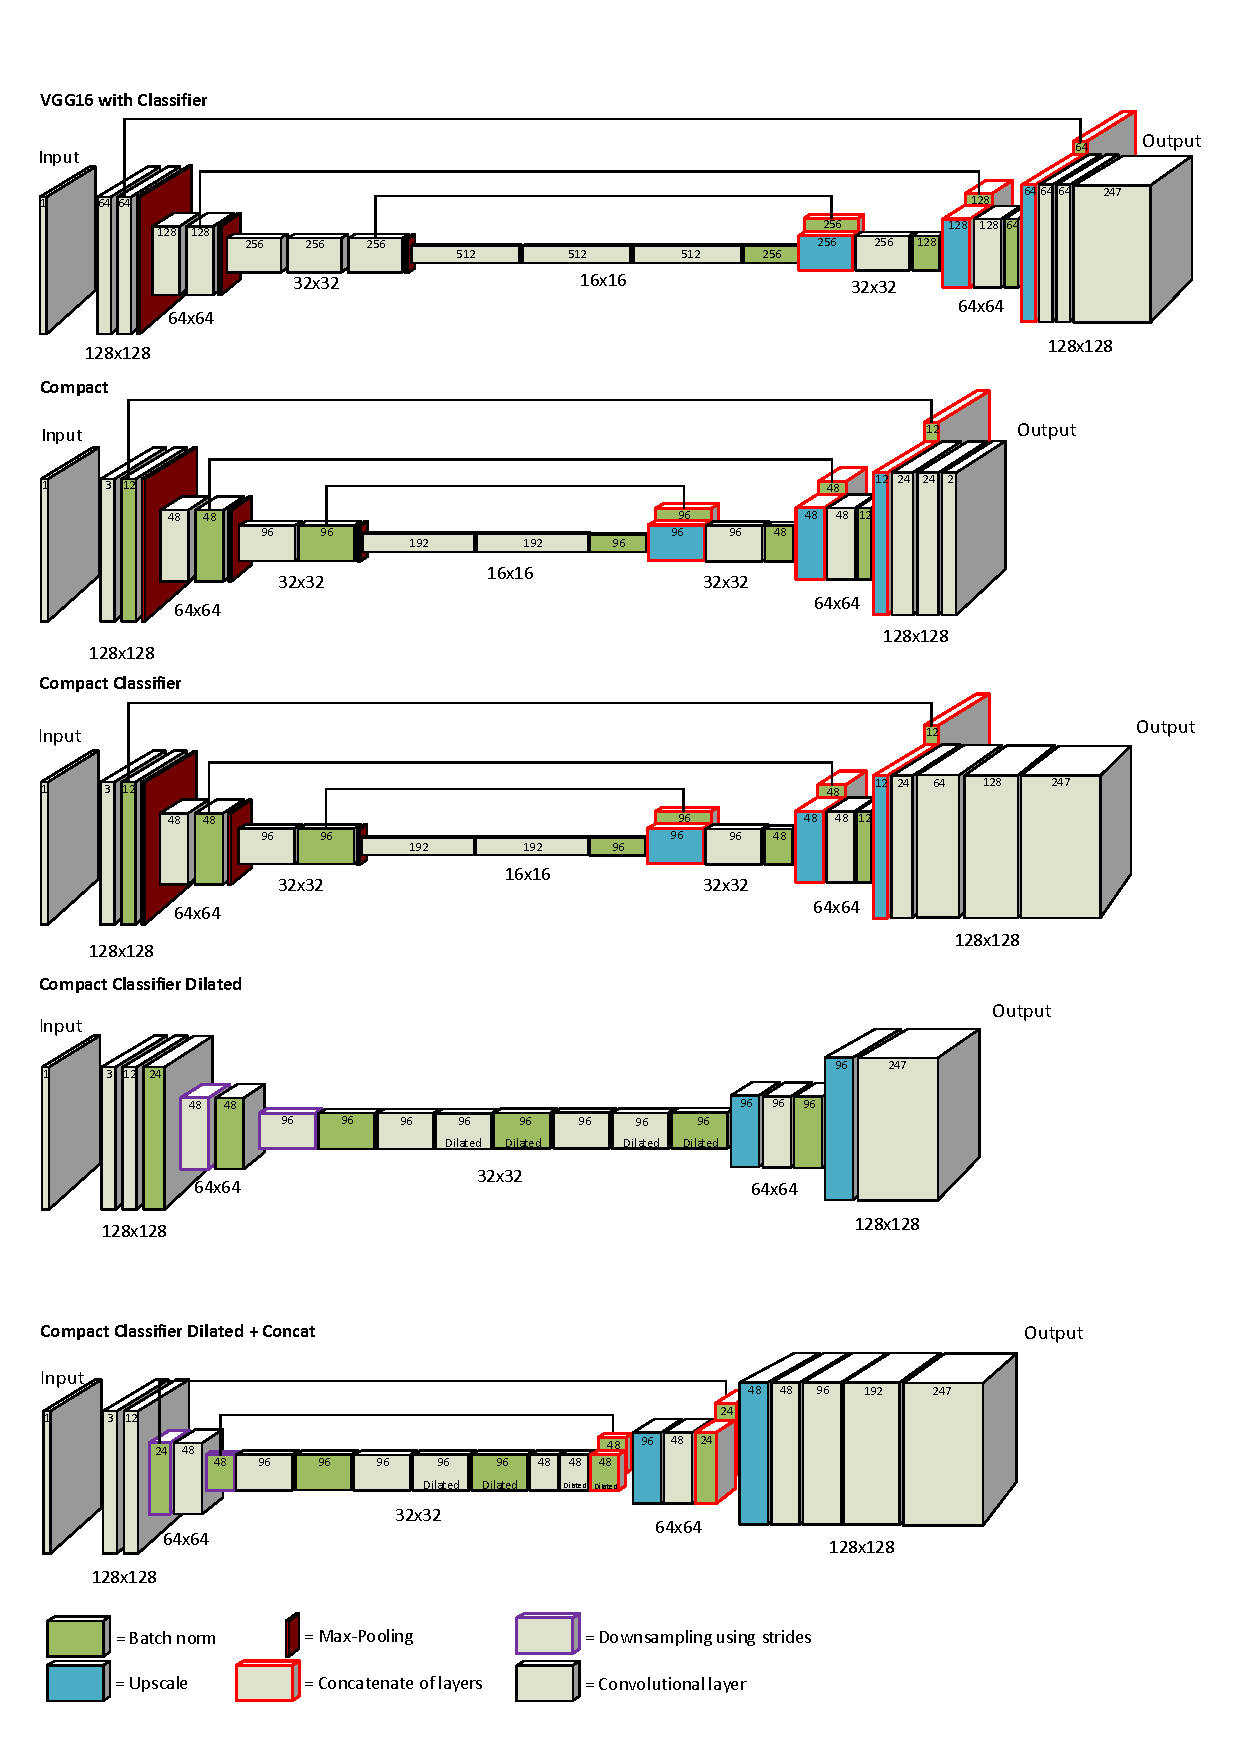
\includegraphics[width=0.95\textwidth,trim={0cm 13.5cm 0.5cm 11.4cm},clip]{final_architecture.pdf}
	\caption{The compact classifier network architecture. The definition of each different layer can be found in figure \ref{fig:Legend}.}
	\label{fig:compact_classifier}
\end{figure}

\subsubsection{Compact classifier dilated}
The compact classifier dilated removes the max-pool layers and the concatenation layers, but instead uses stride to downscale in the feature extraction layers, to maintain the spatial information, and dilation in the reconstruction layer. The dilation gives a better receptive field and thus reduces the need to use subsequent convolutional layers. The classifier is still used and therefore the out put of the network are again the number of colorbins. The network architecture is illustrated in figure \ref{fig:compact_classifier_dilated}.
\begin{figure}[H]
	\centering
	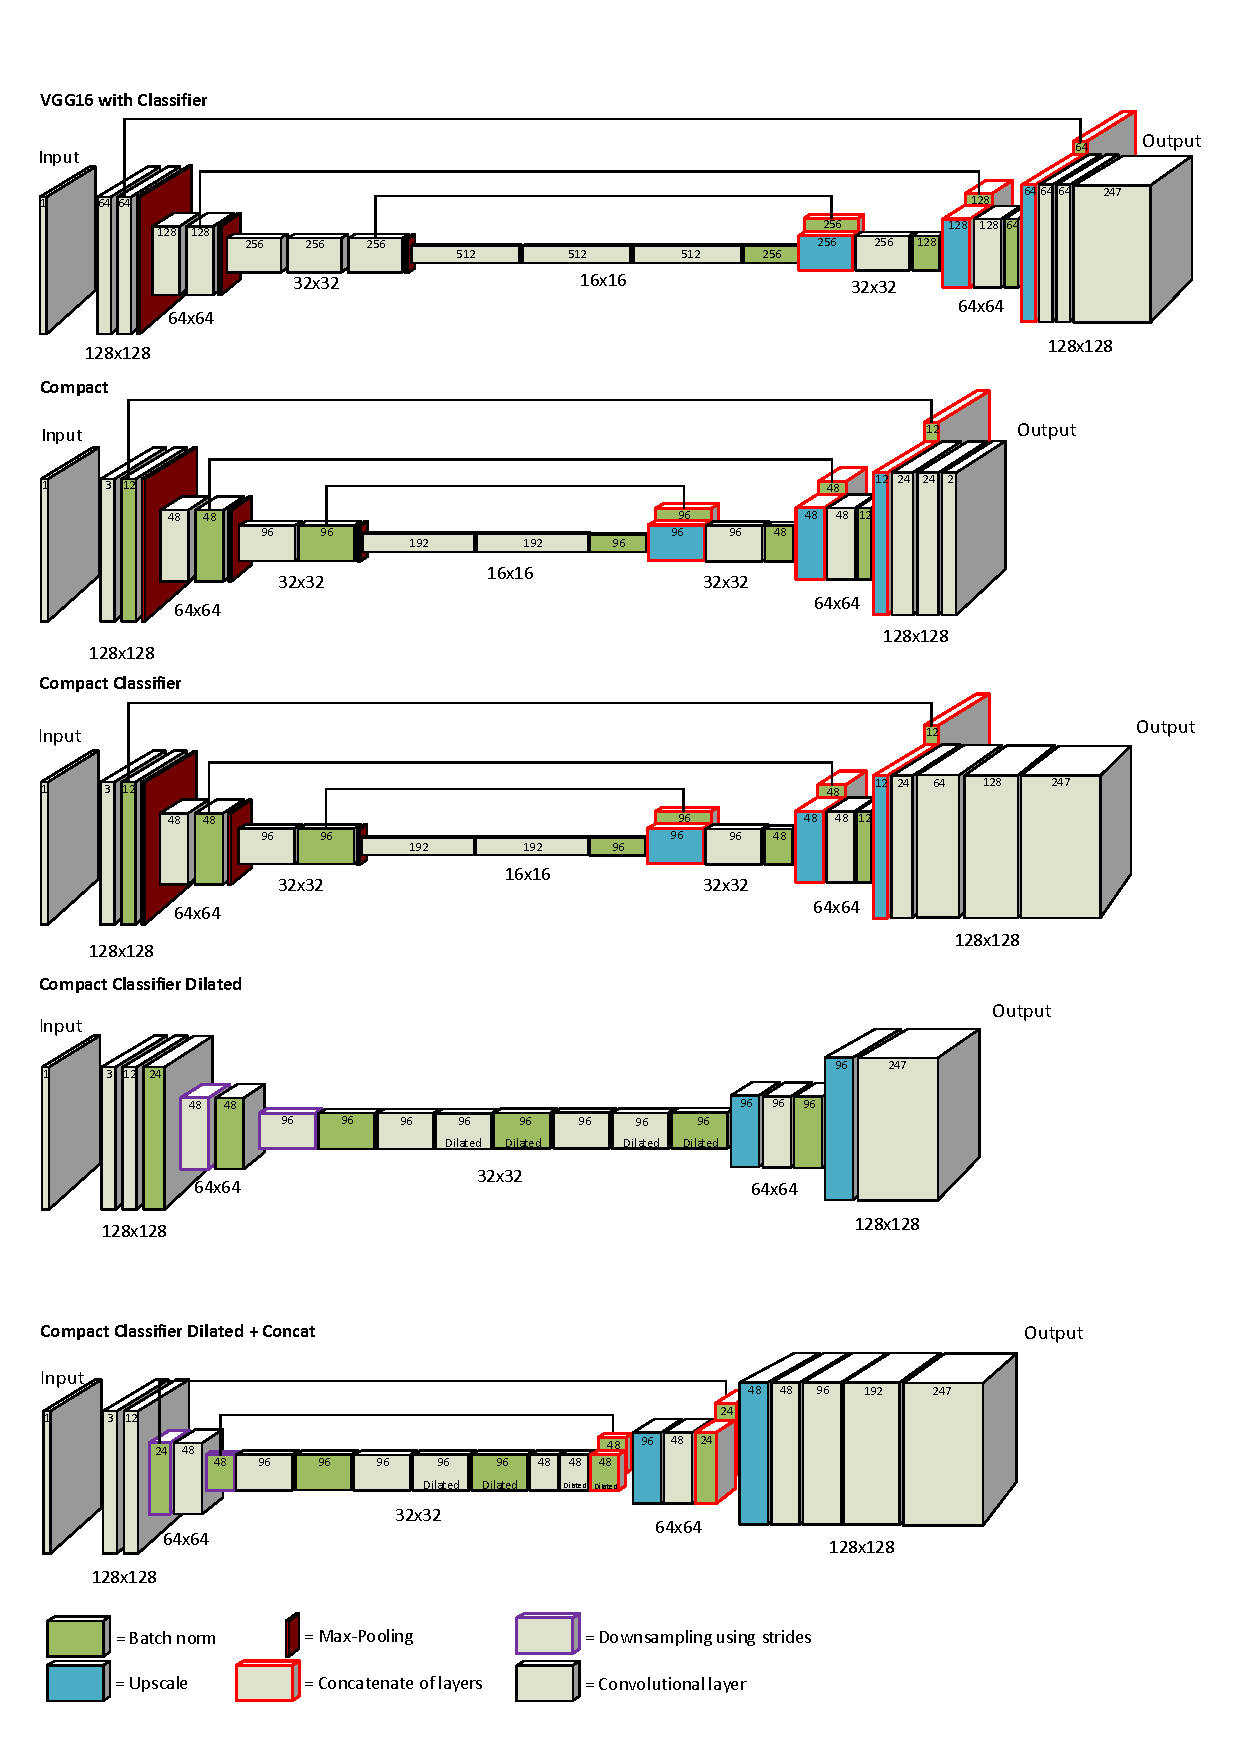
\includegraphics[width=0.95\textwidth,trim={0cm 8.5cm 3cm 16.5cm},clip]{final_architecture.pdf}
	\caption{The compact classifier dilated network architecture. The definition of each different layer can be found in figure \ref{fig:Legend}.}
	\label{fig:compact_classifier_dilated}
\end{figure}

\subsubsection{Compact classifier dilated and concat}
This network not only uses dilated convolutions but adds concatenation of the feature extraction network with the reconstruction network to add more spatial information. The network architecture is illustrated in figure \ref{fig:compact_classifier_dilated_concat}.
\begin{figure}[H]
	\centering
	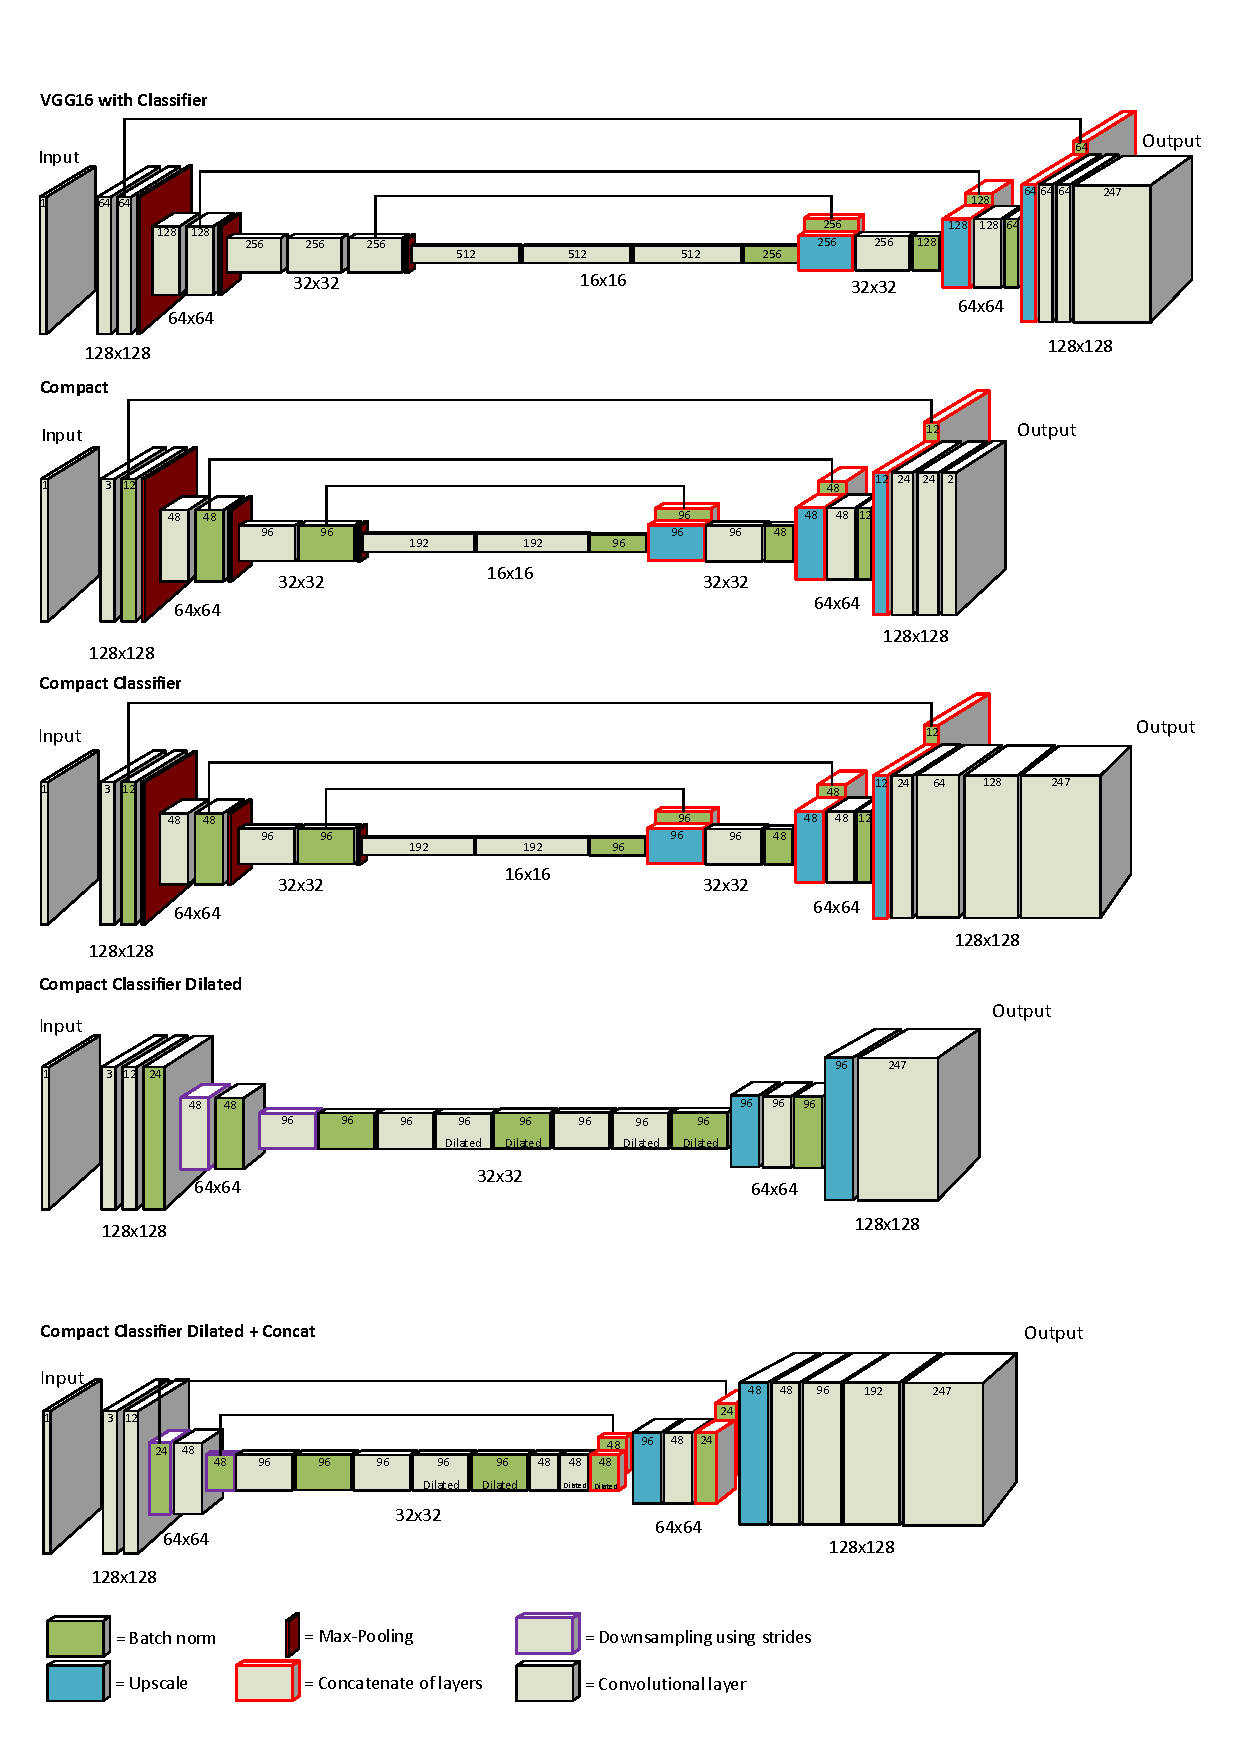
\includegraphics[width=0.95\textwidth,trim={0cm 2.5cm 2.5cm 21.5cm},clip]{final_architecture.pdf}
	\caption{The compact classifier dilated + concat network architecture. The definition of each different layer can be found in figure \ref{fig:Legend}.}
	\label{fig:compact_classifier_dilated_concat}
\end{figure}


\subsubsection{VGG16 classifier}
The VGG16 compact classifier is the same network as the compact classifier, but instead uses the weights of the VGG16 network for the feature extraction part of the network, also making these weights non-trainable. VGG16 does not use batch normalization, therefore each layer that is concatenated is copied (having shared non-trainable weights) and the batch normalization is applied on the copied layer before the nonlinearity. The network architecture is illustrated in figure \ref{fig:VGG_classifier}.
\begin{figure}[H]
	\centering
	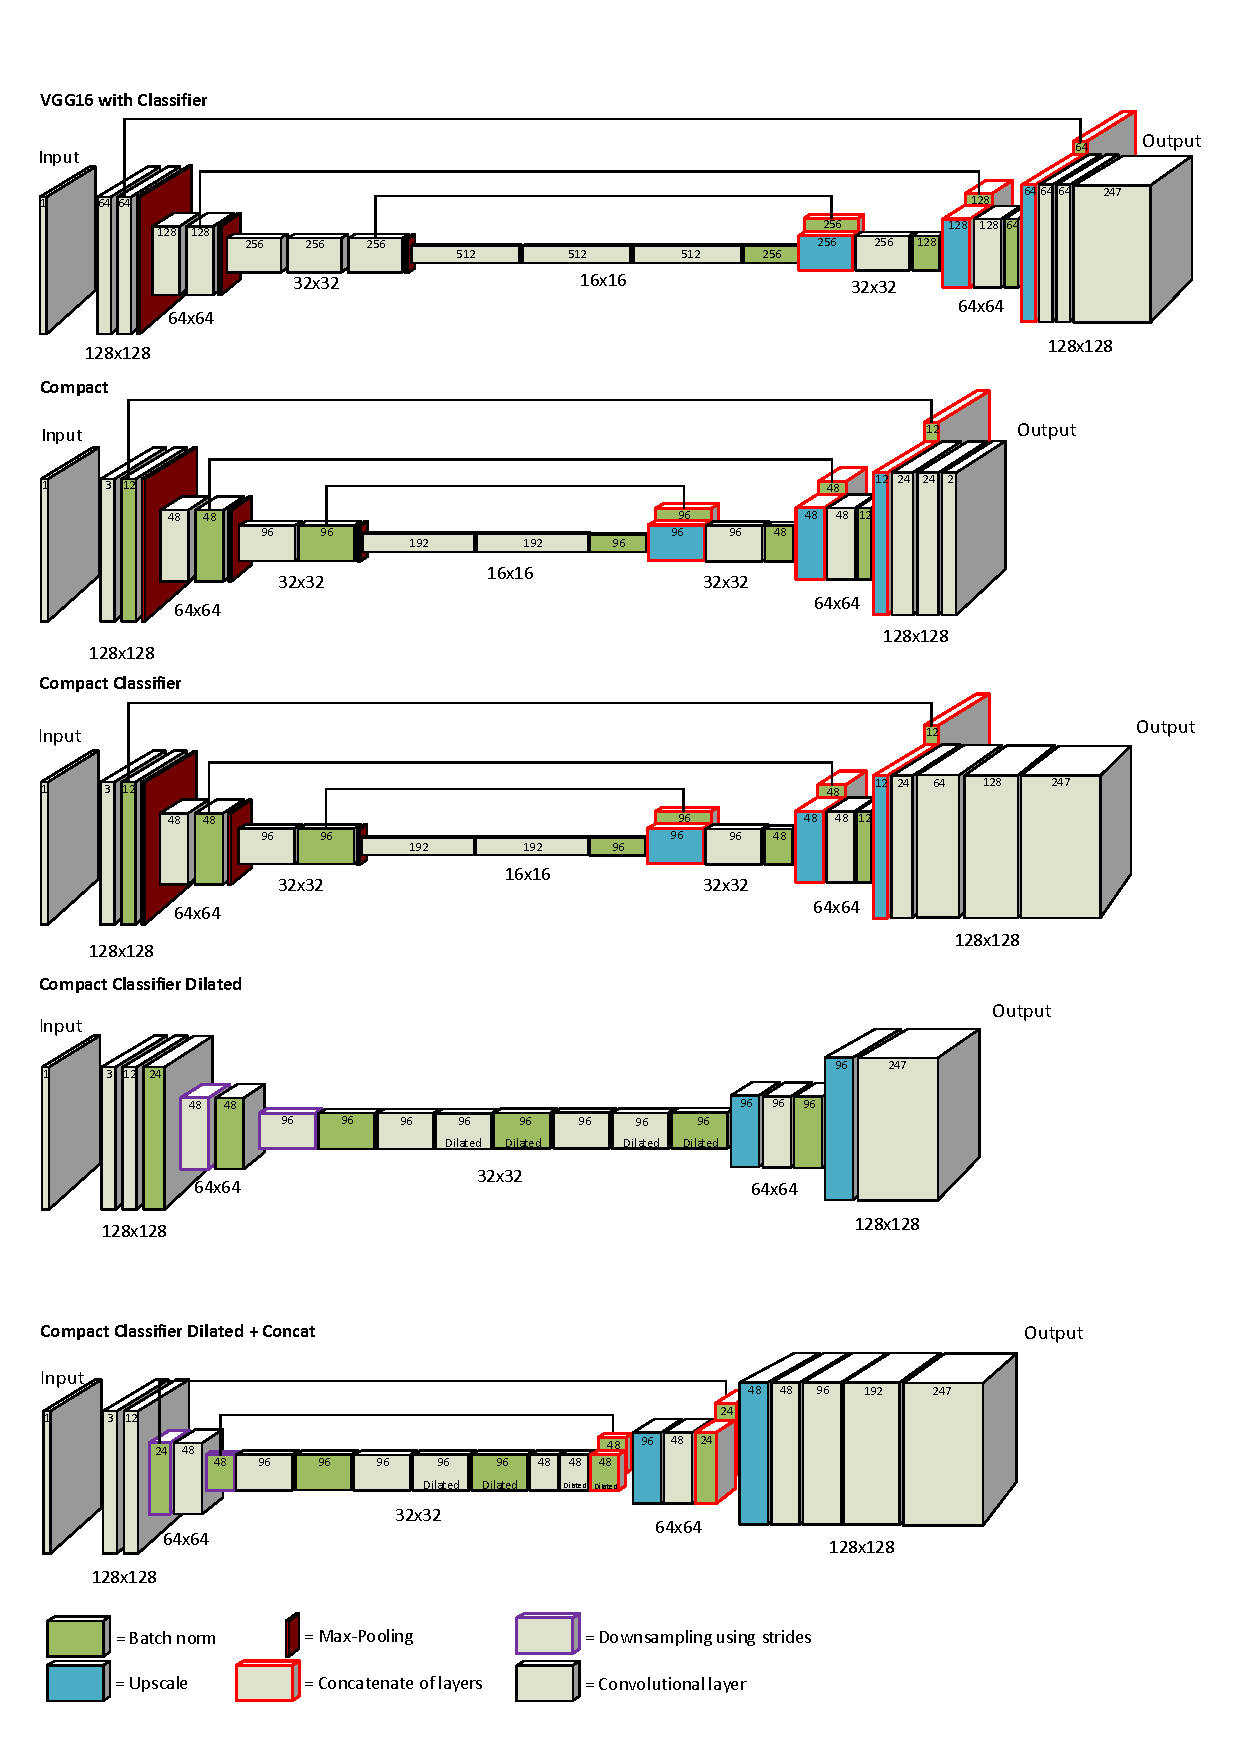
\includegraphics[width=0.95\textwidth,trim={0cm 23.5cm 0.5cm 1.5cm},clip]{final_architecture.pdf}
	\caption{The VGG16 classifier network architecture. The definition of each different layer can be found in figure \ref{fig:Legend}.}
	\label{fig:VGG_classifier}
\end{figure}







